\documentclass[10pt,a4paper]{article}
\usepackage[utf8]{inputenc}
\usepackage[english]{babel}
\usepackage[T1]{fontenc}
\usepackage{amsmath}
\usepackage{amsfonts}
\usepackage{amssymb}
\usepackage{graphicx}
\usepackage{listings}
\usepackage{upgreek}

\author{Milan Tepic, Ivan Antunovic, Peter von Zameck Glyscinski}
\title{Assignment 4 Team 5}
\bibliographystyle{plain}

\begin{document}
\maketitle
\section*{Task 1}
\subsection*{a)}
\begin{figure}[h]
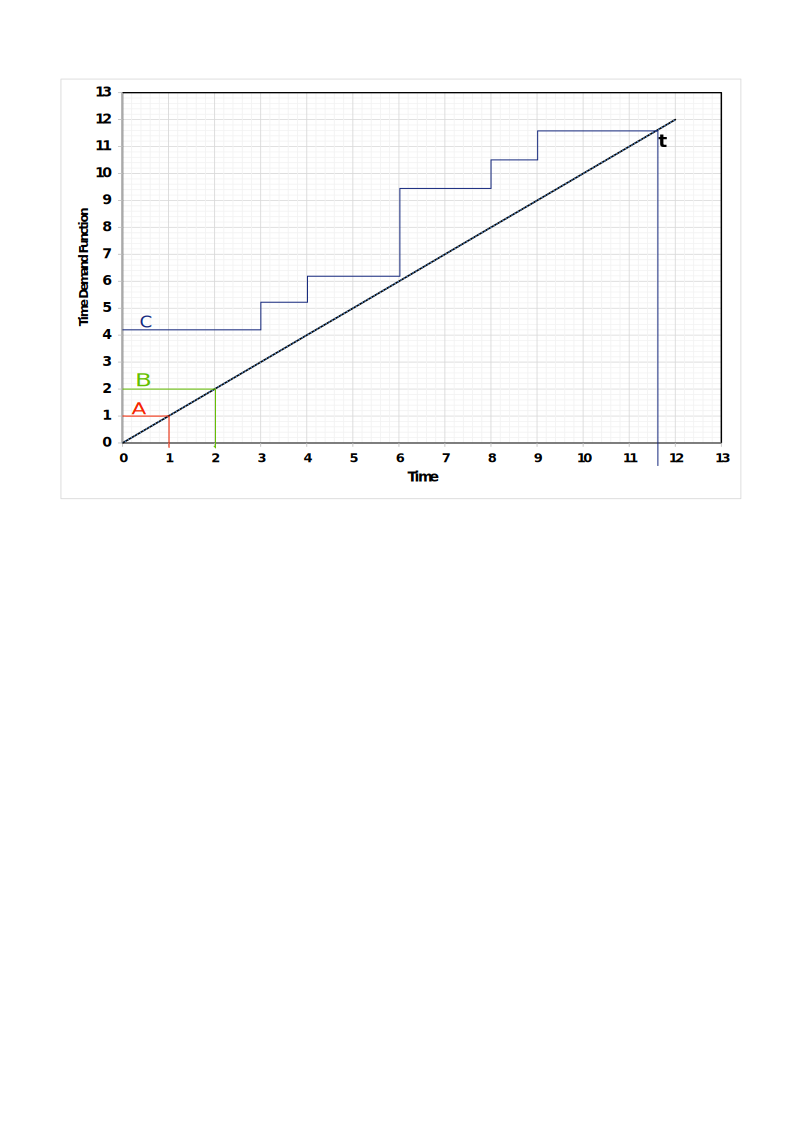
\includegraphics[width=\linewidth]{time-demand-1a.pdf}
\caption{Time demand diagram.} 
\label{fig:1a}
\end{figure}
At t = 1, task A intersects with a line, since deadline of task A is at t = 3, task A fulfills the deadline. Task B intersects with line at t = 2, since deadline of task B is at t = 4, task B fulfills its deadline. Task C intersects with a line before the end of hyper period at t 0 = 12, task C meets its deadline. Thus whole task set T1 is schedulable.

\subsection*{b)}

\begin{figure}[h]
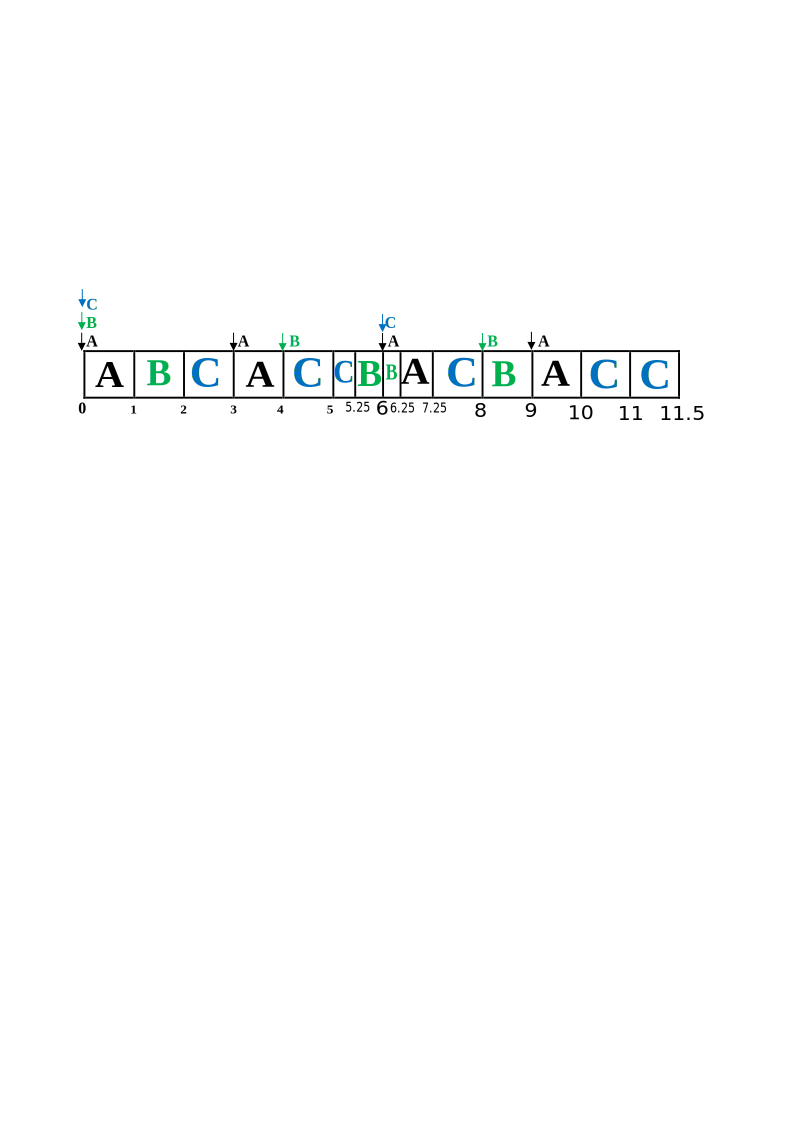
\includegraphics[width=\linewidth]{1b-edf.pdf}
\caption{Timing diagram with EDF.} 

\textbf{NOTE: At time t=3 for EDF diagram, task A is scheduled not task C (both have same deadline, thus alphabetic order is used), please correct the the diagram. Also task C ends at $t=11.5$ not at $t=12$}
\newline 


\label{fig:1bedf}
\end{figure}

\begin{figure}[h]
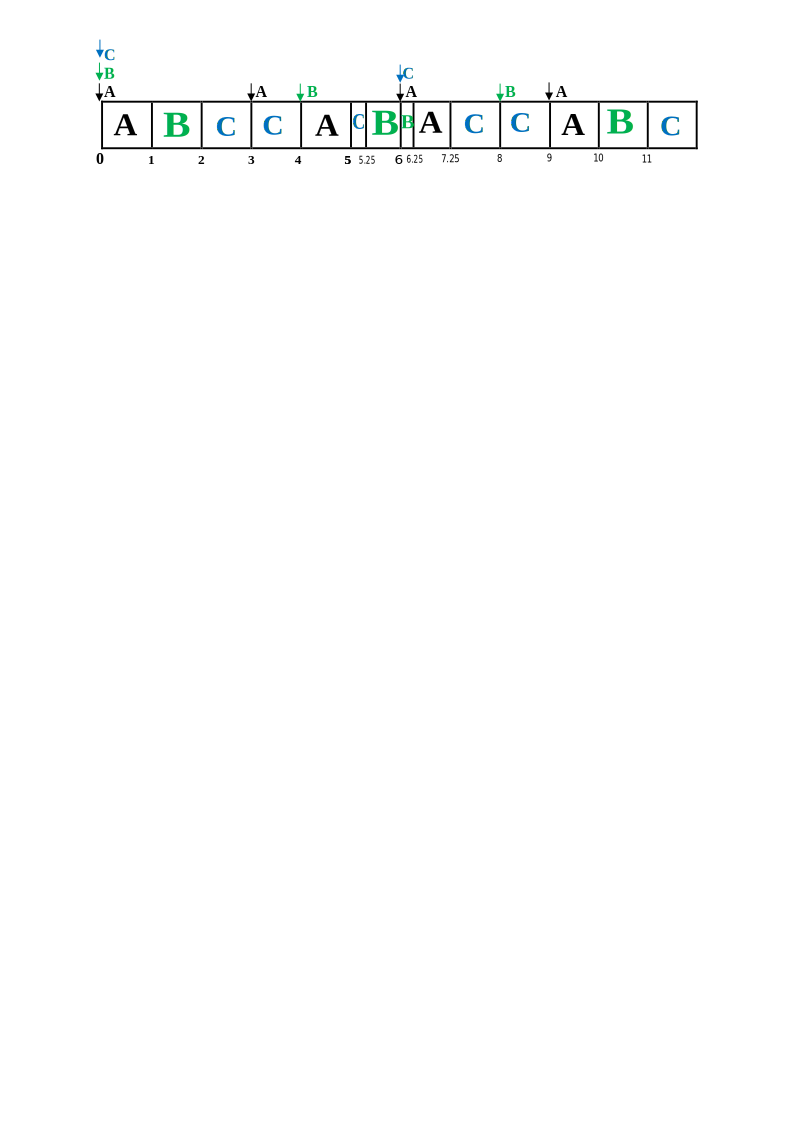
\includegraphics[width=\linewidth]{1b-lst.pdf}
\caption{Timing diagram with LST.} 
\label{fig:1blst}
\end{figure}

\textbf{TODO: In timing diagram for LST, task C executes until t = 12. However at t = 11.5 task C should stop executing.}

\textbf{TODO: Please correct timing diagram for LST. Task C should stop executing at $t=11.5$}

\begin{center}
\caption {LST Scheduling table} \label{tab:lst} 
 \begin{tabular}
 {||c c c c||} 
 \hline
 t & $s_A$ & $s_B$ & $s_C$ \\ [0.5ex] 
 \hline\hline
 0 & $3-0-1=2$ & $4-0-1=3$ & $6-0-2.25=3.75$ \\ 
 \hline
 1 & $/$ & $4-1-1=2$ & $6-1-2.25=2.75$ \\
 \hline
 2 & $/$ & $/$ & $6-2-2.25=1.75$ \\
 \hline
 3 & $3-0-1=2$ & $/$ & $6-3-1.25=1.75$ \\
 \hline
 4 & $3-1-1=1$ & $4-0-1=3$ & $6-4-0.25=1.75$ \\
 \hline
 5 & $/$ & $4-1-1=2$ & $6-5-0.25=0.75$ \\
 \hline
 5.25 & $/$ & $4-1.25-1=1.75$ & $/$ \\
 \hline
 6 & $3-0-1=2$ & $4-2-0.25=1.75$ & $6-0-2.25=3.75$ \\
 \hline
 6.25 & $3-0.25-1=1.75$ & $/$ & $6-0.25-2.25=3.5$ \\
 \hline
 7 & $3-1-0.25=1.75$ & $/$ & $6-1-2.25=2.75$ \\
 \hline
 7.25 & $/$ & $/$ & $6-1.25-2.25=2.5$ \\
 \hline
 8 & $/$ & $4-0-1=3$ & $6-2-1.5=2.5$\\ \hline
 9 & $3-0-1=2$ & $4-1-1=2$ & $6-3-0.5=2.5$\\
 \hline
 10 & $/$ & $4-2-1=1$ & $6-4-0.5=1.5$\\
 \hline
 11 & $/$ & $/$ & $6-5-0.5=0.5$ \\
 [1ex] 
 \hline
\end{tabular}
\end{center}

Table above \ref{tab:lst} shows calculation of slack times. Given a task $T_i = (p_i,r_i,e_i,d_i)$, its slack time is defined as Given a task $s_i = (d_i - t) - e_i'$, where t is the time elapsed since the start of the current cycle, and $e_i' \leq e_i$ is its remaining demand for execution time \cite{Fan:2015:RES:2800613}.
\subsection*{c)}

\begin{figure}[h]
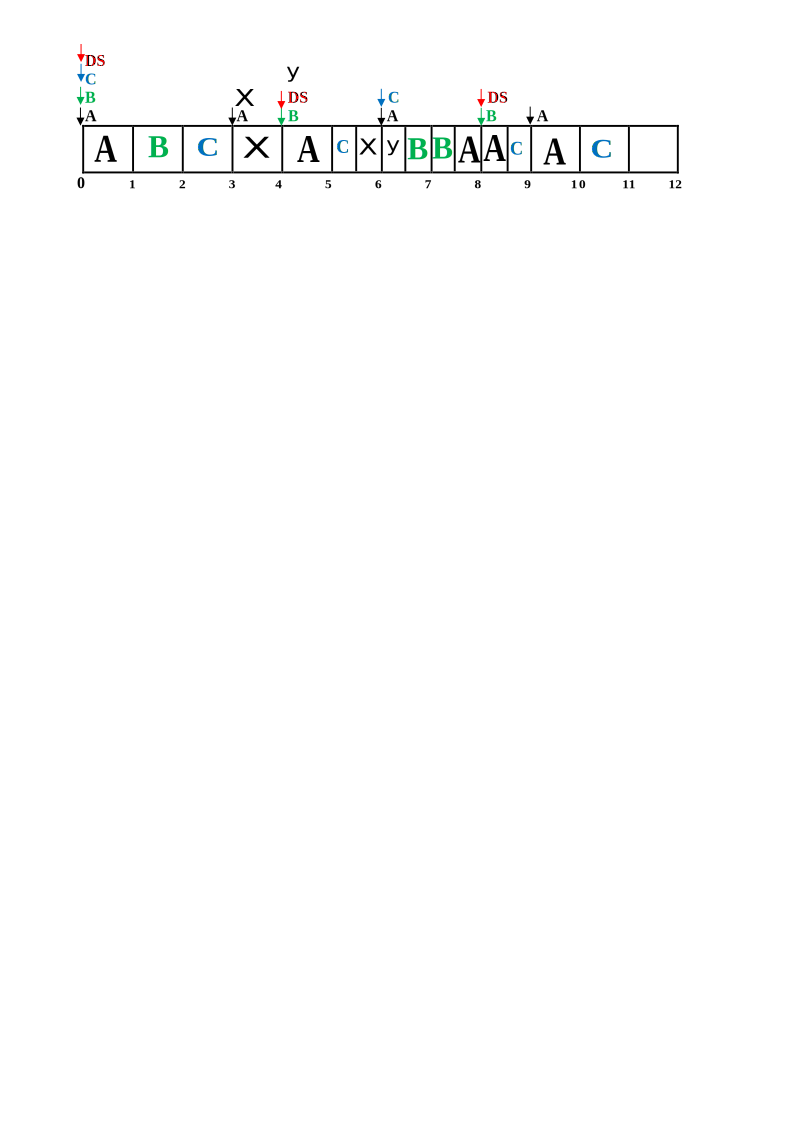
\includegraphics[width=\linewidth]{1c.pdf}
\caption{Timming diagramm with aperiodic tasks.} 
\label{fig:1c}
\end{figure}
\newpage

\textbf{At t=8.5 task B is executed until t =9, in your diagram task C instead is executed}

\begin{itemize}
  \item At $t=0$ there are no aperiodic tasks in the queue, hence we execute task A using EDF algorithm. Same is for tasks B, C, executed at time 2, 3 respectively. 
  \item At $t=3$ aperiodic task X and periodic task A are released. Server gets executed and compares deadline of task A ($t=6$) and server ($t=4$). Because server has earlier deadline, it gets scheduled according to EDF.
  \item At $t=4$ the execution budget of a server is replenished again. We make decision based on EDF again. Since task A has earliest deadline it is executed.
\begin{center}
 \begin{tabular}{|c|c|c|c|}
   \hline
    t & $T_{DS}$ & $T_A$ & $T_B$ \\
    \hline
    4 & 8 & 6 & 8 \\
    \hline
 \end{tabular}
\end{center}

\item At $t=5.5$, we finish execution of $T_C$ and we make EDF decision again. Since both task $T_DS$ and $T_B$ have equal deadlines, deferrable server is scheduled first (given in the task). Thus aperiodic task $X$ is executed since it arrived earlier than aperiodic task $Y$. 
\begin{center}
 \begin{tabular}{|c|c|c|c|}
   \hline
    t & $T_{DS}$ & $T_B$  \\
    \hline
    4 & 8 & 8 \\
    \hline
 \end{tabular}
\end{center}

\item At $t=6$ we make another scheduling decision. Server has already used 0.5 time units, and has still 0.5 left in the current period. The \textit{deferrable server} has earlier deadline at $t=8$ and aperiodic task $Y$ gets executed.
\begin{center}
 \begin{tabular}{|c|c|c|c|}
   \hline
    t & $T_{DS}$ & $T_A$ & $T_C$ \\
    \hline
    6 & 8 & 9 & 12 \\
    \hline
 \end{tabular}
\end{center}

\item At $t=6.5$ aperodic task $Y$ finishes its execution. No further aperiodic tasks arrive, thus remaining tasks are scheduled according to EDF.
\end{itemize}



\section*{Task 2}
\subsection*{a)}
\begin{tabular}{|c|c|c|c|}
\hline
    Context & Timer 1 & Timer 2 & Timer 3 \\
    \hline
    Context 1 & $\overline{w_{39}}$ ~in ~$i_4$ & $\overline{w_{51}}$ ~in ~$i_4$ & $\overline{w_0}$ ~in ~$i_4$ \\
    \hline
    Context 2 & $\overline{w_{9}}$ ~in ~$i_1$ &  $\overline{w_{51}}$ ~in ~$i_4$ & $\overline{w_0}$ ~in ~$i_4$ \\
    \hline
    Context 3 & - &  $\overline{w_{51}}$ ~in ~$i_4$ & $\overline{w_0}$ ~in ~$i_4$ \\
    \hline
    Context 4 & - & - &  $\overline{w_{27}}$ ~in ~$i_3$\\
    \hline
\end{tabular}

\section*{Task 3}

\subsection*{a)}
\textbf{TODO: finish part a)}
\subsection*{b)}
At the start and end of an ISR, interrupts are disabled during context switching, to ensure that enough context of the processor has been saved onto the interrupt stack. If interrupts are not disabled in these cases, further interrupts could change the unsaved context (e.g. changing values of commonly used registers) of interrupted program. Once the ISR  has  run to completion, the control returns back to the original program that was suspended, now commonly used registers contain different values than the ones prior to the interrupt. Program will continue executing unexpectedly.
\subsection*{c)}
\begin{figure}[h]
\includegraphics[width=\linewidth]{3c.pdf}
\caption{Vectored Interrupt Handling.} 
\label{fig:1c}
\end{figure}
\newpage

\section*{Task 4}
\subsection*{a)}
Upper priority bound is assigned to every semaphore (priority ceiling). This upper bound is the priority of the task with the highest priority that uses this semaphore.
\begin{enumerate}
    \item $C(A) = max\{Pri(T_{2}), Pri(T_{3}), Pri(T_{4})\} = Pri(T_2) = 4$
    \item $C(B) = max\{Pri(T_{1}), Pri(T_{3}), Pri(T_{4})\} = Pri(T_1) = 5$
    \item $C(C) = max\{Pri(T_{1}), Pri(T_{2})\} = Pri(T_1) = 5$
\end{enumerate}
,where $C(X)$ denotes priority ceiling of semaphore X.
The table for ICP is shown below.
\begin{center}
 \begin{tabular}{||c c c c c c||} 
 \hline
 t & $\overset{\mathrm{\wedge}}{\Pi}(t)$ & $\pi_1(t)$
 & $\pi_2(t)$ & $\pi_3(t)$ & $\pi_4(t)$  \\ [0.5ex] 
 \hline\hline
 0 & $\Omega$ & 5 & 4 & 3 & 2 \\ 
 \hline
 1 & $\Omega$ & 5 & 4 & 3 & 2 \\
 \hline
 2 & $\Omega\rightarrow4$& 5 & 4 & 3 & 2  \\
 \hline
 3 & $4$ & 5 & 4 & 3 & 2  \\
 \hline
 4 & $4$ & 5 & 4 & 3 & $2\rightarrow4$  \\
 \hline
 5 & $4\rightarrow5$ & 5 & 4 & 3 & 4  \\
 \hline
 6 & $5$ & 5 & 4 & 3 & 4  \\
 \hline
 7 & $5\rightarrow4$ & 5 & 4 & 3 & 4  \\
 \hline
 8 & $4$ & 5 & 4 & 3 & 4  \\
 \hline
 9 & $4\rightarrow5$ & 5 & 4 & 3 & $4\rightarrow2$ \\
 \hline
 10 & $5$ & 5 & 4 & 3 & $2$ \\
 \hline
 11 & $5$ & 5 & $4\rightarrow5$ & 3 & $2$ \\
 \hline
 12 & $\Omega\rightarrow5$ & 5 & $5\rightarrow4$ & 3 & 2 \\
 \hline
 13 & $5$ & 5 & 4 & 3 & 2 \\
 \hline
 14 & $5$ & 5 & 4 & 3 & 2 \\
 \hline
 15 & $5\rightarrow\Omega$ & 5 & 4 & 3 & 2 \\
 \hline
 16 & $\Omega$ & 5 & 4 & 3 & 2 \\
 \hline
 17 & $\Omega$ & 5 & 4 & 3 & 2 \\
 \hline
 18 & $\Omega\rightarrow4$ & 5 & 4 & 3 & 2 \\
 \hline
 19 & $4\rightarrow\Omega$ & 5 & 4 & 3 & 2 \\
 \hline
 20 & $\Omega$ & 5 & 4 & 3 & 2 \\
 \hline
 21 & $\Omega$ & 5 & 4 & 3 & 2 \\
 \hline
 22 & $\Omega\rightarrow5$ & 5 & 4 & 3 & 2 \\
 \hline
 23 & $5$ & 5 & 4 & 3 & 2 \\
 \hline
 24 & $5$ & 5 & 4 & 3 & 2 \\
 \hline
 25 & $5$ & 5 & 4 & 3 & 2 \\
 \hline
 26 & $5$ & 5 & 4 & 3 & 2 \\
 \hline
 27 & $5\rightarrow\Omega$ & 5 & 4 & 3 & 2 \\
 \hline
 28 & $\Omega$ & 5 & 4 & 3 & 2 \\
 \hline
 29 & $\Omega$ & 5 & 4 & 3 & 2 \\
 [1ex] 
 \hline
\end{tabular}
\end{center}

$\pi_i$ is the current priority of task \textit{i}.
At any time t, the current priority ceiling $\overset{\mathrm{\wedge}}{\Pi}(t)$ of the system is equal to the highest priority ceiling of the resources that are in use at the time.

\begin{figure}[h]
\includegraphics[width=\linewidth]{4a.pdf}
\caption{Timing diagram for Priority Ceiling Protocol.} 
\label{fig:4a}
\end{figure}

\begin{enumerate}
    \item At $t=4$ $T_2$ tries to acquire $S_C$, task $T_2$ gets blocked because $4=\pi_2\not\>\pi_4=4$. $T_A$ starts executing as it is only ready task. $T_2$ transmits its active priority to the task $T_4$ that holds the semaphore $S_C$.
    \item At $t=5$ $T_3$ gets ready, since $3=\pi_3\not>\pi_4=4$, $T_4$ has higher priority and starts executing.
    \item At $t=9$, the $T_4$ releases $S_A$, its active priority becomes its nominal priority.\textbf{
    The rule is that 
    the task that blocks other task and inherits its priority, executes at its inherited priority until the time when it releases every resource whose priority ceiling is equal to or higher than inherited priority $\pi(t)$}.
    Since $T_4$ does not lock any resource, and it returns to its nominal priority. Now $T_2$ has higher priority than $T_3$ and $T_4$ and it starts to execute at $t=9$.
    \item At $t=10$ the task $T_1$ becomes ready and as highest priority task it starts to execute.
    \item At $t=11$,  $5=\pi_5(t)\not>\overset{\mathrm{\wedge}}{\Pi}(t)=5$, thus $T_1$ gets blocked by $T_2$ (because $T_2$ has locked $S_C$). $T_1$ transmits its active priority to the task $T_2$. And $T_2$ resumes execution with its inherited priority $\pi_1(t)=5$.
    \item At $t=12$, $T_2$ unlocks $S_C$ and its active priority is set to its nominal priority. $T_1$ is unblocked and as a result, $T_1$ starts executing. No resources are locked by any other tasks, thus $T-1$ is granted access to the $S_B$.
    \item At $t=14$, similar to $t=12$ $T_2$ again is granted access to the resource, since no other tasks hold the any resources.
    \item At $t=16$, task $T_1$ finishes its execution, and $T_2$ is executed because of its highest priority.
    \item At $t=18$,  $T_2$ is granted access to the resource $S_A$, since no other tasks hold any resources.
    \item At $t=20$, $T_2$ finishes its execution and $T_3$ is executed as it has higher priority than $T_4$.
    \item At $t=2$,  $T_3$ is granted access to the resource $S_B$, since no other tasks hold any resources.
    \item At $t=23$, $T_3$ tries to grant access to $S_A$. Now we have situation where $3=\pi_3(t)\not>\overset{\mathrm{\wedge}}{\Pi}(t)=5$, but since $T_3$ is the job holding the resource whose priority ceiling is equal to $\overset{\mathrm{\wedge}}{\Pi}(t)$. In other words $T_3$ is only task that currently uses resources ($S_B$ is locked by $T_3$), thus $T_3$ cannot run into the deadlock situation. Access for $S_A$ is granted to $T_3$.
    \item At $t=28$, $T_3$ runs to completion. Now $T_4$ is the only ready task and it executes until $t=29$ when it finishes its execution. 
\end{enumerate}


\subsection*{b)}
Below table shows priorities for ICPP.
\begin{center}
 \begin{tabular}{||c c c c c c||} 
 \hline
 t & $\overset{\mathrm{\wedge}}{\Pi}(t)$ & $\pi_1(t)$
 & $\pi_2(t)$ & $\pi_3(t)$ & $\pi_4(t)$  \\ [0.5ex] 
 \hline\hline
 0 & $\Omega$ & 5 & 4 & 3 & 2 \\ 
 \hline
 1 & $\Omega$ & 5 & 4 & 3 & 2 \\
 \hline
 2 & $4$& 5 & 4 & 3 & 4  \\
 \hline
 3 & $4$ & 5 & 4 & 3 & 4  \\
 \hline
 4 & $4$ & 5 & 4 & 3 & 4  \\
 \hline
 5 & 5 & 5 & 4 & 3 & 5  \\
 \hline
 6 & $5$ & 5 & 4 & 3 & 5  \\
 \hline
 7 & $5$ & 5 & 4 & 3 & 4  \\
 \hline
 8 & $5$ & 5 & 4 & 3 & 4  \\
 \hline
 9 & $5$ & 5 & 5 & 3 & 2 \\
 \hline
 10 & $5$ & 5 & 5 & 3 & 2 \\
 \hline
 11 & $\Omega$ & 5 & 4 & 3 & 2 \\
 \hline
 12 & $5$ & 5 & 5 & 3 & 2 \\
 \hline
 13 & $\Omega$ & 5 & 4 & 3 & 2 \\
 \hline
 14 & $5$ & 5 & 4 & 3 & 2 \\
 \hline
 15 & $\Omega$ & 5 & 4 & 3 & 2 \\
 \hline
 16 & $\Omega$ & 5 & 4 & 3 & 2 \\
 \hline
 17 & $\Omega$ & 5 & 4 & 3 & 2 \\
 \hline
 18 & $4$ & 5 & 4 & 3 & 4 \\
 \hline
 19 & $\Omega$ & 5 & 4 & 3 & 4 \\
 \hline
 20 & $\Omega$ & 5 & 4 & 3 & 2 \\
 \hline
 21 & $\Omega$ & 5 & 4 & 3 & 2 \\
 \hline
 22 & $5$ & 5 & 4 & 5 & 2 \\
 \hline
 
 23 & $5$ & 5 & 4 & 5 & 2 \\
 \hline
 24 & $5$ & 5 & 4 & 5 & 2 \\
 \hline
 25 & $5$ & 5 & 4 & 5 & 2 \\
 \hline
 26 & $5$ & 5 & 4 & 5 & 2 \\
 \hline
 27 & $\Omega$ & 5 & 4 & 3 & 2 \\
 \hline
 28 & $\Omega$ & 5 & 4 & 3 & 2 \\
 \hline
 29 & $\Omega$ & 5 & 4 & 3 & 2 \\
 [1ex] 
 \hline
\end{tabular}
\end{center}
 
  \begin{figure}[h]
\includegraphics[width=\linewidth]{4b.pdf}
\caption{Timing diagram for Immediate Ceiling Priority Protocol.}
\label{fig:4b}
\end{figure}
\newpage

 \begin{enumerate}
     \item At $t=5$ $T_3$ becomes ready, but it cannot execute because $3=\pi_3\not\>\pi_4=5$
     \item At $t=9$ $T_4$ unlocks $S_A$, priority of $T_4$ is set to its nominal priority (4).
     Task $T_2$ which was blocked on semaphore $S_A$ gets activated.
     $T_2$ acquires semaphore $S_C$ since no other semaphore is locked.
     \item At $t=10$ $T_1$ is active, but active priority of $T_2$ is equal to nominal priority of $T_1$ ($5 = Pri(T_2) = Pri(T_1) = 5$). In PIP and ICPP tasks with same priority are executed according to the FIFO policy, thus $T_2$ continues its execution.
     \item At $t=11$ $T_2$ releases $S_C$, and its priority is set to nominal priority. Now task $T_1$ being highest priority task is executed. 
     \item At $t=12$ since no resource is being used by other tasks, $T_1$ acquires $S_B$.
     \item At $t=14$ since no resource is being used by other tasks, $T_1$ acquires $S_C$.
     \item At $t=16$ $T_1$ finishes its execution. Now $T_2$ is the ready task with highest priority, and it starts executing.
     \item At $t=18$ since no resource is being used by other tasks, $T_2$ acquires $S_C$.
     \item At $t=20$ $T_2$ finishes its execution. Now $T_3$ is the ready task with highest priority, and it starts executing.
     \item At $t=22$ since no resource is being used by other tasks, $T_2$ acquires $S_B$.
     \item At $t=28$ $T_3$ finishes its execution. Now $T_4$ is the only ready task and it starts its execution.
     
 \end{enumerate}
 
\bibliographystyle{plain}
\bibliography{references}
\end{document}